\section{Results}\label{sec:results}

\subsection{General noise}

\begin{figure}[!tbp]
    \centering
        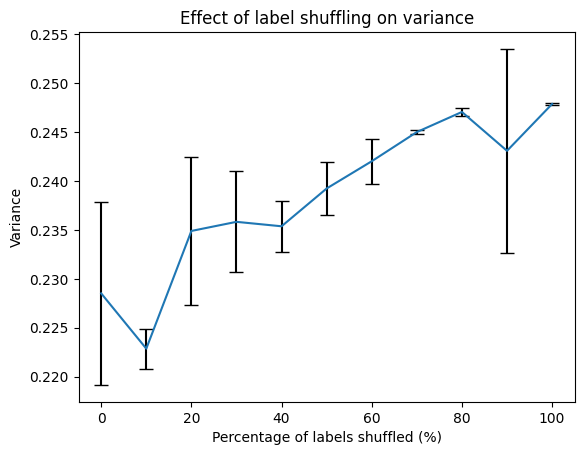
\includegraphics[width=7.7cm]{img/label_shuffle.png}
    \caption{The average non-ErrP and ErrP signal on the FcZ channel. These signals originate from subject 1 during session 1.}
    \label{fig:label_shuffle}
\end{figure}

\begin{figure}[!tbp]
    \centering
        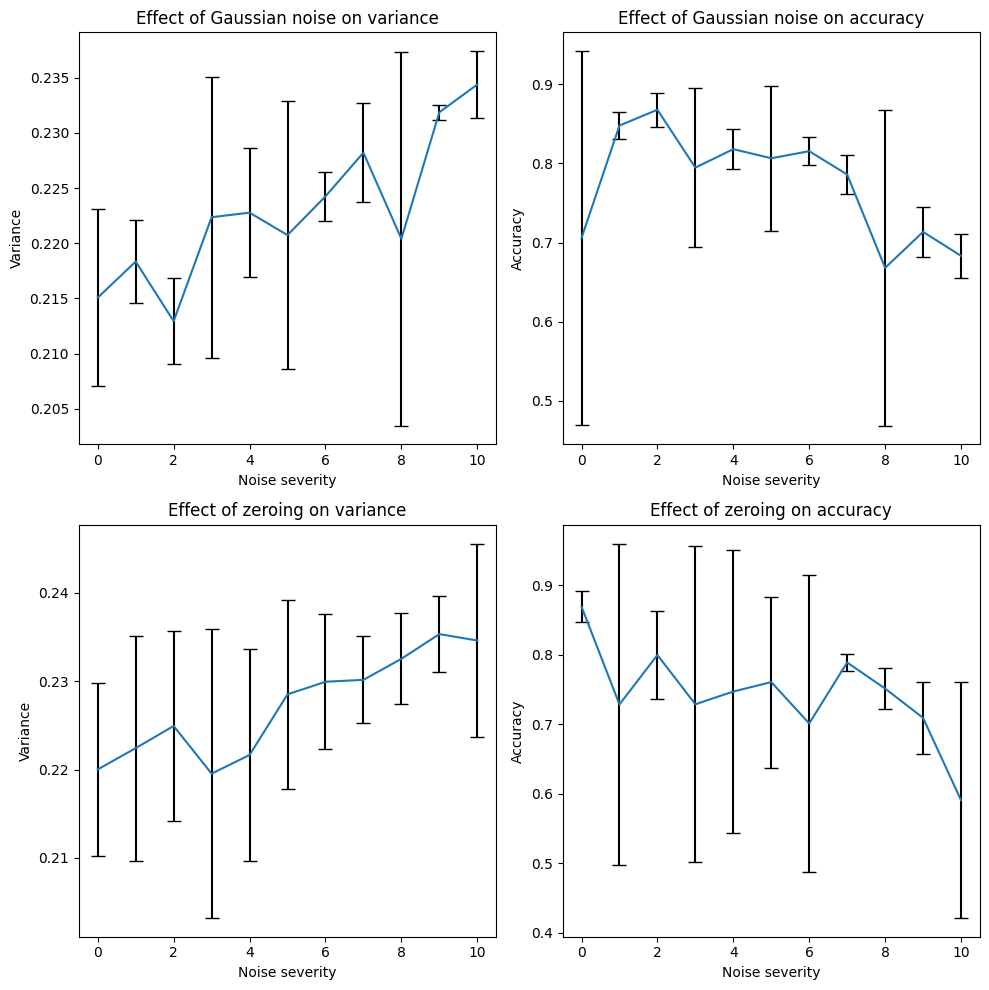
\includegraphics[width=7.7cm]{img/general.png}
    \caption{The average non-ErrP and ErrP signal on the FcZ channel. These signals originate from subject 1 during session 1.}
    \label{fig:general}
\end{figure}

\subsection{Localized noise}

\begin{figure}[!tbp]
    \centering
        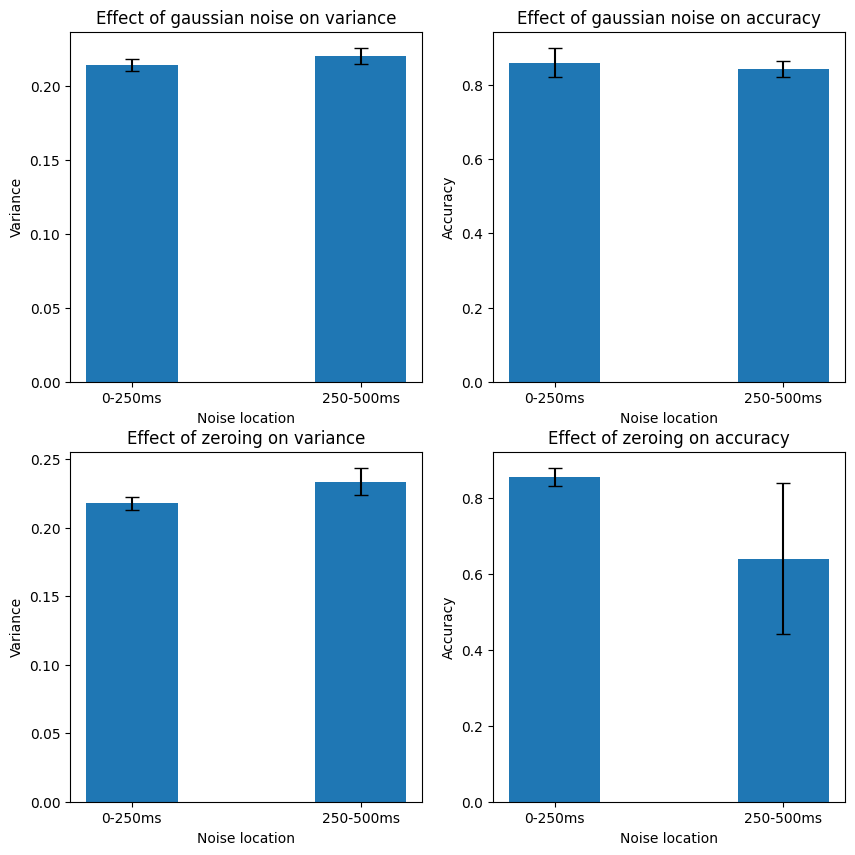
\includegraphics[width=7.7cm]{img/local.png}
    \caption{The average non-ErrP and ErrP signal on the FcZ channel. These signals originate from subject 1 during session 1.}
    \label{fig:local}
\end{figure}

\subsection{Tracable noise}

\begin{figure}[!tbp]
    \centering
        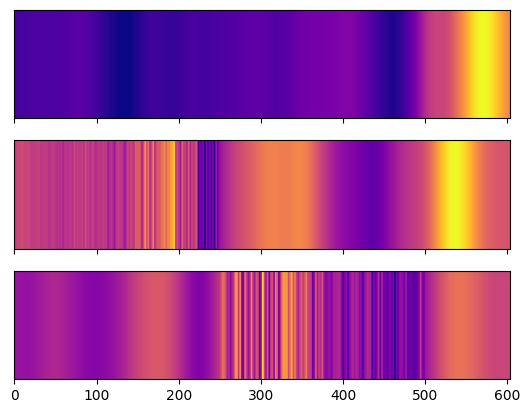
\includegraphics[width=7.7cm]{img/gaussian_shap.png}
    \caption{The average non-ErrP and ErrP signal on the FcZ channel. These signals originate from subject 1 during session 1.}
    \label{fig:gaussian_shap}
\end{figure}

\begin{figure}[!tbp]
    \centering
        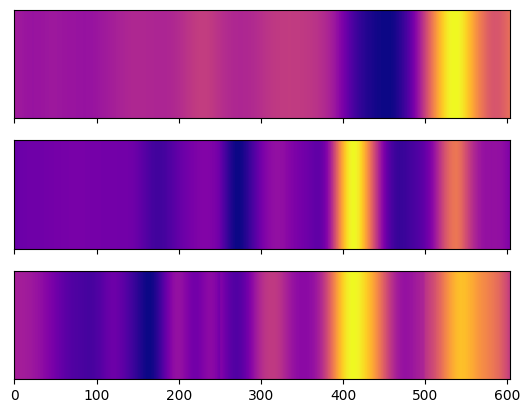
\includegraphics[width=7.7cm]{img/zeroed_shap.png}
    \caption{The average non-ErrP and ErrP signal on the FcZ channel. These signals originate from subject 1 during session 1.}
    \label{fig:zeroed_shap}
\end{figure}